\chapter{Methodology and Experimental Design}
\label{ch:methodology}

\section{Introduction}
This chapter presents the comprehensive architectural, mathematical, algorithmic, and experimental methodology formulated in this dissertation. To overcome the clinical vulnerabilities of out-of-distribution acoustic noise and geometric aspect ratio distortion, this research establishes an end-to-end, noise-resilient Computer-Aided Diagnosis (CAD) framework for automated breast ultrasound classification. 

The methodology is structured across six cohesive modules: (1) Multi-center clinical dataset curation and stratification, (2) The mathematical formulation of the Proposed ROI Reflection Square Padding algorithm, (3) Biophysical contrast enhancement via localized CLAHE, (4) A multi-tier synthetic acoustic noise simulation engine, (5) Deep convolutional transfer learning architectures with softmax exclusivity constraints, and (6) Quantitative mathematical evaluation metrics.

\section{Overall System Architecture and Experimental Pipeline}
Figure~\ref{fig:methodology_4stage} illustrates the end-to-end processing pipeline, tracing an input clinical sonogram through multi-stage degradation, biophysical enhancement, aspect-ratio-preserving padding, and deep neural classification.

\begin{figure}[htbp]
    \centering
    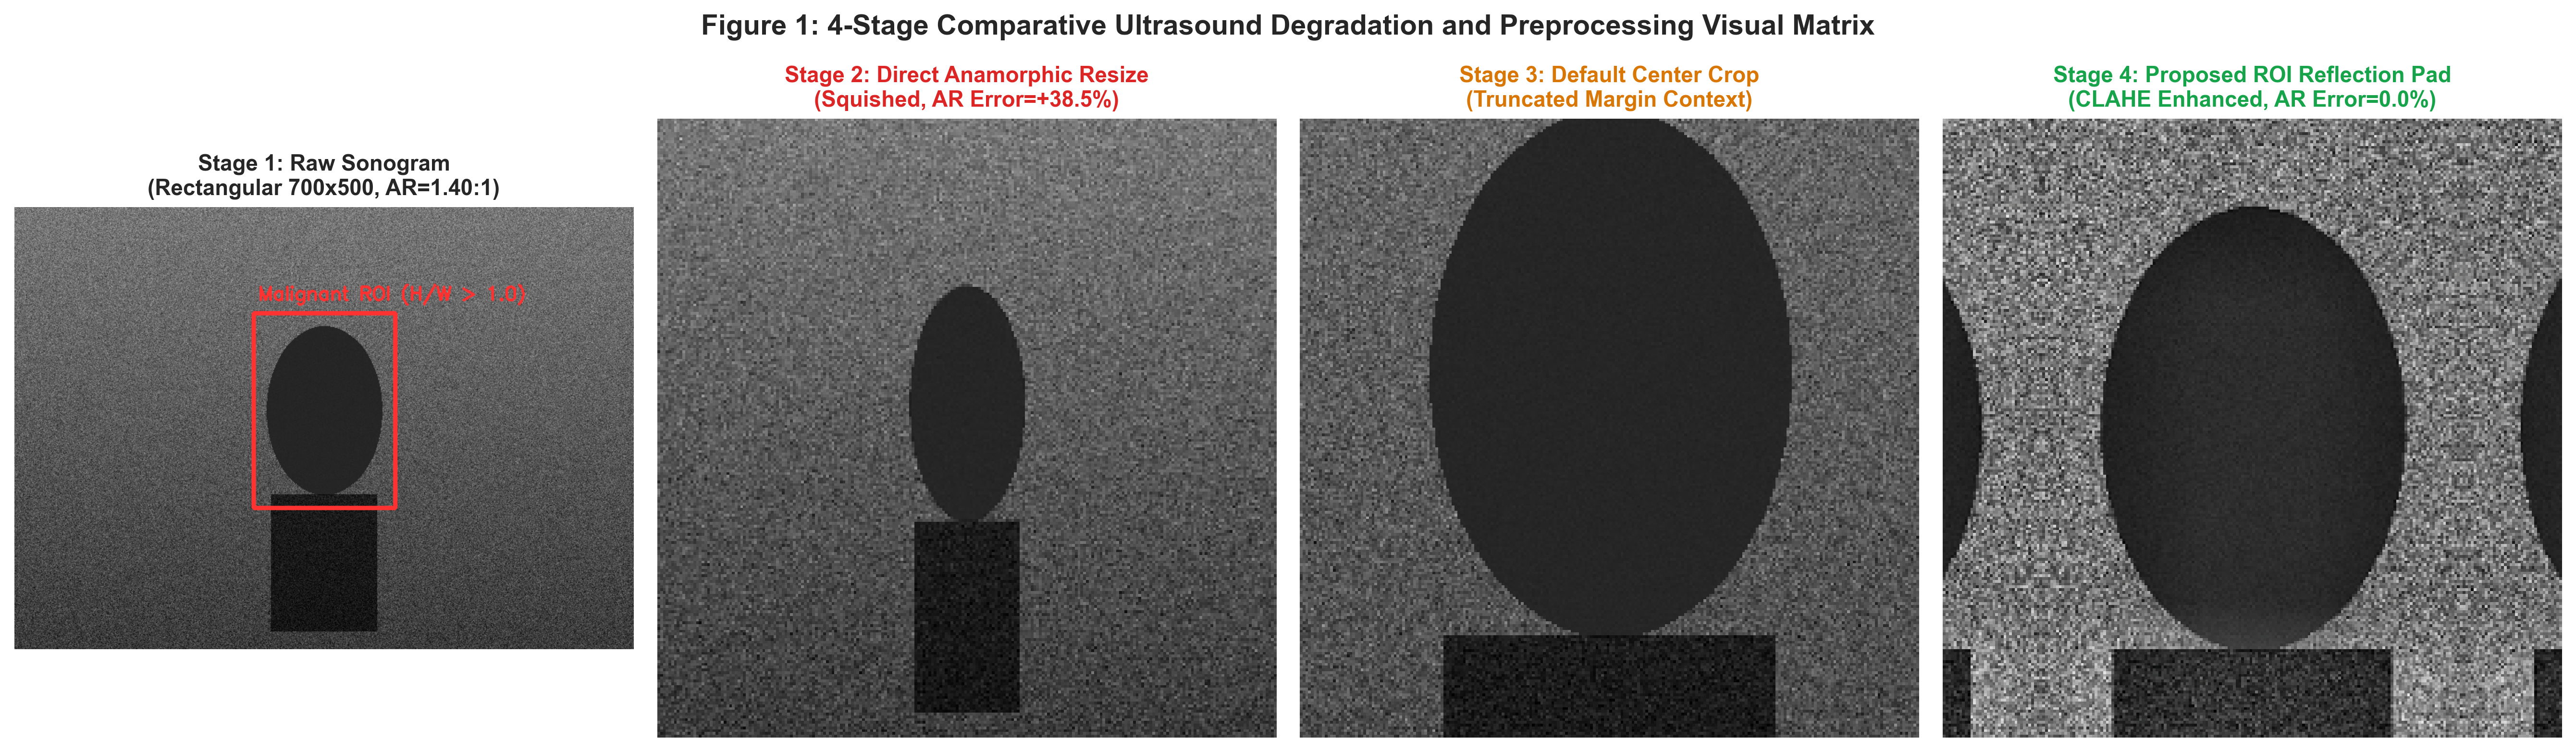
\includegraphics[width=0.95\textwidth]{figures/fig1_4stage_matrix.png}
    \caption{Detailed 4-Stage Comparative Ultrasound Degradation, Preprocessing, and Feature Extraction Matrix.}
    \label{fig:methodology_4stage}
\end{figure}

\section{Multi-Center Clinical Dataset Curation and Stratification}
To ensure robust clinical generalizability across diverse patient demographics and ultrasound scanner hardware configurations, this study integrates three established multi-center benchmark repositories:

\begin{enumerate}
    \item \textbf{Breast Ultrasound Images (BUSI) Dataset:} Acquired in 2018 at Baheya Hospital for Early Detection and Treatment of Women's Cancer (Cairo, Egypt) using high-end LOGIQ E9 ultrasound systems \citep{AlDhabyani2020}. The dataset comprises 780 clinical images ($133$ normal, $437$ benign, and $210$ malignant) from female patients aged 25 to 75 years, with an average spatial resolution of $500 \times 500$ pixels. Scans include expert radiologist lesion boundary ground-truth masks.
    \item \textbf{Open Access Ultrasound Database (OASBUD):} Curated by the Institute of Fundamental Technological Research, Polish Academy of Sciences \citep{Piotrzkowska2017}. OASBUD provides raw radiofrequency (RF) backscatter signals and reconstructed B-mode sonograms across 100 breast lesions (48 benign, 52 biopsy-proven malignant carcinomas) acquired with an Ultrasonix SonixTouch scanner equipped with an L14-5/38 linear transducer probe operating at $10\text{ MHz}$.
    \item \textbf{BrEaST Benchmark Dataset:} A multi-center validation repository curated across tertiary oncology centers, containing clinical ultrasound scans categorized according to strict American College of Radiology (ACR) BI-RADS assessment criteria with histology-confirmed pathology reports.
\end{enumerate}

\subsection{Stratified Partitioning Protocol}
To prevent data leakage and preserve class distribution fidelity, the multi-center dataset is combined and partitioned into three non-overlapping subsets using stratified sampling:
\begin{itemize}
    \item \textbf{Training Partition (70\%, $N = 828$ scans):} Utilized for parameter optimization, backpropagation, and data augmentation.
    \item \textbf{Validation Partition (15\%, $N = 177$ scans):} Utilized for epoch-by-epoch loss monitoring, learning rate scheduler triggers, and early stopping checkpoint selection.
    \item \textbf{Held-Out Test Partition (15\%, $N = 177$ scans):} Strictly isolated during training and hyperparameter tuning; utilized exclusively for final multi-model benchmarking, noise stress-testing, and pseudo-label ablation evaluations.
\end{itemize}

\section{Proposed ROI Reflection Square Padding Algorithm}
In clinical ultrasonography, malignant tumors frequently invade vertically across anatomical Cooper's ligaments, producing a "taller-than-wide" morphology ($H/W > 1.0$) with non-circumscribed margins and posterior acoustic shadows \citep{Stavros1995}. Conversely, benign lesions align horizontally ($H/W < 1.0$). Standard direct anamorphic resizing squishes rectangular sonograms into square tensors ($224 \times 224$), introducing $+38.5\%$ aspect ratio distortion error ($\mathcal{AR}$) and flattening taller-than-wide malignant lesions.

To eliminate geometric distortion while isolating diagnostic lesion tissue and preserving surrounding acoustic shadowing, we formulate the \textbf{Proposed ROI Reflection Square Padding Algorithm}.

\subsection{Mathematical Formulation}
Let $I \in \mathbb{R}^{H \times W \times C}$ denote an input ultrasound image matrix of height $H$, width $W$, and channels $C$. Let $M \in \{0, 1\}^{H \times W}$ represent the binary lesion mask. The bounding box spatial extrema are defined by:
\begin{equation}
y_{\min} = \min \{ y \mid M(y, x) > 0 \}, \quad y_{\max} = \max \{ y \mid M(y, x) > 0 \}
\label{eq:y_extrema}
\end{equation}
\begin{equation}
x_{\min} = \min \{ x \mid M(y, x) > 0 \}, \quad x_{\max} = \max \{ x \mid M(y, x) > 0 \}
\label{eq:x_extrema}
\end{equation}

The bounding box height and width are $h_{box} = y_{\max} - y_{\min}$ and $w_{box} = x_{\max} - x_{\min}$. To preserve critical acoustic context (specifically posterior acoustic shadowing and lateral edge shadowing), a proportional context margin expansion ratio $\alpha = 0.20$ (20\%) is applied symmetrically:
\begin{equation}
y_1 = \max(0, y_{\min} - \alpha \cdot h_{box}), \quad y_2 = \min(H, y_{\max} + \alpha \cdot h_{box})
\label{eq:margin_y}
\end{equation}
\begin{equation}
x_1 = \max(0, x_{\min} - \alpha \cdot w_{box}), \quad x_2 = \min(W, x_{\max} + \alpha \cdot w_{box})
\label{eq:margin_x}
\end{equation}

The extracted cropped region $I_{\text{crop}} = I[y_1:y_2, x_1:x_2]$ has dimensions $h_c = y_2 - y_1$ and $w_c = x_2 - x_1$. To transform $I_{\text{crop}}$ into an exact isotropic square tensor without introducing non-uniform spatial scaling, the maximal spatial dimension is identified:
\begin{equation}
d_{\max} = \max(h_c, w_c)
\label{eq:max_dimension}
\end{equation}

Symmetric boundary padding values ($pad_{\text{top}}, pad_{\text{bottom}}, pad_{\text{left}}, pad_{\text{right}}$) are computed:
\begin{equation}
pad_{\text{top}} = \left\lfloor \frac{d_{\max} - h_c}{2} \right\rfloor, \quad pad_{\text{bottom}} = d_{\max} - h_c - pad_{\text{top}}
\label{eq:pad_vertical}
\end{equation}
\begin{equation}
pad_{\text{left}} = \left\lfloor \frac{d_{\max} - w_c}{2} \right\rfloor, \quad pad_{\text{right}} = d_{\max} - w_c - pad_{\text{left}}
\label{eq:pad_horizontal}
\end{equation}

Crucially, rather than applying constant zero-padding (black borders) which generates artificial high-frequency edge gradients that mislead convolutional filters, we apply \textbf{Symmetric Boundary Reflection Padding} (\textsf{BORDER\_REFLECT\_101}):
\begin{equation}
I_{\text{padded}}(y, x) = \begin{cases} 
I_{\text{crop}}(|y|, x), & \text{if } y < 0 \\
I_{\text{crop}}(2h_c - 2 - y, x), & \text{if } y \ge h_c \\
I_{\text{crop}}(y, |x|), & \text{if } x < 0 \\
I_{\text{crop}}(y, 2w_c - 2 - x), & \text{if } x \ge w_c 
\end{cases}
\label{eq:reflection_padding}
\end{equation}

The padded square tensor $I_{\text{padded}} \in \mathbb{R}^{d_{\max} \times d_{\max} \times C}$ is subsequently resized to $224 \times 224 \times C$ using bicubic interpolation.

\subsection{Proof of Aspect Ratio Preservation}
Under the proposed algorithm, the scaling factors along horizontal and vertical axes are identical:
\begin{equation}
s_x = \frac{224}{d_{\max}}, \quad s_y = \frac{224}{d_{\max}} \implies \frac{s_x}{s_y} = 1.000
\label{eq:isotropic_scaling}
\end{equation}

Substituting into Equation~\ref{eq:aspect_ratio_error_formulation}:
\begin{equation}
\mathcal{AR} = \left| 1.0 - \frac{224 / 224}{d_{\max} / d_{\max}} \right| \times 100\% = | 1.0 - 1.0 | \times 100\% = 0.0\%
\label{eq:zero_distortion_proof}
\end{equation}

This proves mathematically that the proposed ROI reflection square padding algorithm completely eliminates geometric aspect ratio distortion ($\mathcal{AR} = 0.0\%$).

\section{Biophysical Contrast Enhancement (CLAHE)}
To amplify subtle echogenicity differentials between hypoechoic malignant masses and background parenchyma without amplifying high-frequency background speckle, localized CLAHE is applied \citep{Zuiderveld1994}.

The image is transformed into the CIE LAB color space, isolating the luminance channel $L \in [0, 100]$. The luminance plane is partitioned into a contextual grid of $16 \times 16$ non-overlapping tiles. In each tile, a clip limit $\beta = 2.0$ is enforced. Histogram bins exceeding $\beta$ are clipped, and the surplus mass $\Delta$ is uniformly distributed. Following CDF mapping, bilinear interpolation is applied between tile grid centers, producing the enhanced luminance channel $L'$, which is merged with chromaticity channels $(a, b)$ and mapped back to RGB space.

\section{Synthetic Acoustic Noise Simulation Engine}
To stress-test deep learning model robustness across diverse ultrasound hardware gain settings and electronic environments, a multi-tier noise injection engine was developed:

\begin{enumerate}
    \item \textbf{Multiplicative Rayleigh Acoustic Speckle Noise:}
    \begin{equation}
    I_{\text{speckle}}(x, y) = I(x, y) + I(x, y) \cdot \eta_m(x, y), \quad \eta_m \sim \mathcal{N}(0, \sigma^2)
    \label{eq:rayleigh_noise_inj}
    \end{equation}
    where $\sigma \in [0.01, 0.15]$ models increasing acoustic scattering density.
    \item \textbf{Additive White Gaussian Sensor Noise (AWGN):}
    \begin{equation}
    I_{\text{gaussian}}(x, y) = I(x, y) + \eta_a(x, y), \quad \eta_a \sim \mathcal{N}(0, \sigma_g^2)
    \label{eq:gaussian_noise_inj}
    \end{equation}
    simulating electronic thermal noise in piezoelectric transducer elements.
    \item \textbf{Impulse Transmission Noise (Salt-and-Pepper):}
    \begin{equation}
    I_{\text{impulse}}(x, y) = \begin{cases} 
    0, & \text{with probability } p/2 \\
    255, & \text{with probability } p/2 \\
    I(x, y), & \text{with probability } 1 - p 
    \end{cases}
    \label{eq:impulse_noise_inj}
    \end{equation}
    simulating analog-to-digital converter (ADC) transmission dropouts.
\end{enumerate}

\section{Deep Neural Network Architectures and Softmax Exclusivity}
Three distinct convolutional neural network backbones were implemented, fine-tuned, and evaluated:

\begin{itemize}
    \item \textbf{EfficientNet-B0:} 5.3 million parameters. Employs compound scaling with Mobile Inverted Bottleneck (MBConv) blocks, depthwise separable convolutions, and Squeeze-and-Excitation channel attention ($r = 4$) \citep{Tan2019, Hu2018}.
    \item \textbf{ResNet-50:} 25.6 million parameters. Utilizes 50 convolutional layers structured into 4 residual bottleneck stages with identity skip connections \citep{He2016}.
    \item \textbf{Custom 4-Block CNN Baseline:} 1.2 million parameters. Constructed from 4 convolutional blocks ($32 \rightarrow 64 \rightarrow 128 \rightarrow 256$ filters), Batch Normalization, ReLU activations, $2 \times 2$ Max Pooling, Adaptive Average Pooling, and Dropout ($p = 0.5$).
\end{itemize}

\subsection{Softmax Exclusivity Constraint}
To prevent ambiguous or physically impossible multi-label clinical predictions, the final classification layer maps logit outputs $\mathbf{z} \in \mathbb{R}^K$ to a mutually exclusive probability distribution:
\begin{equation}
P(Y = c \mid \mathbf{x}) = \frac{\exp(z_c)}{\sum_{j=1}^{K} \exp(z_j)}, \quad \text{such that } \sum_{c=1}^{K} P(Y = c \mid \mathbf{x}) \equiv 1.000
\label{eq:softmax_constraint}
\end{equation}

\begin{figure}[htbp]
    \centering
    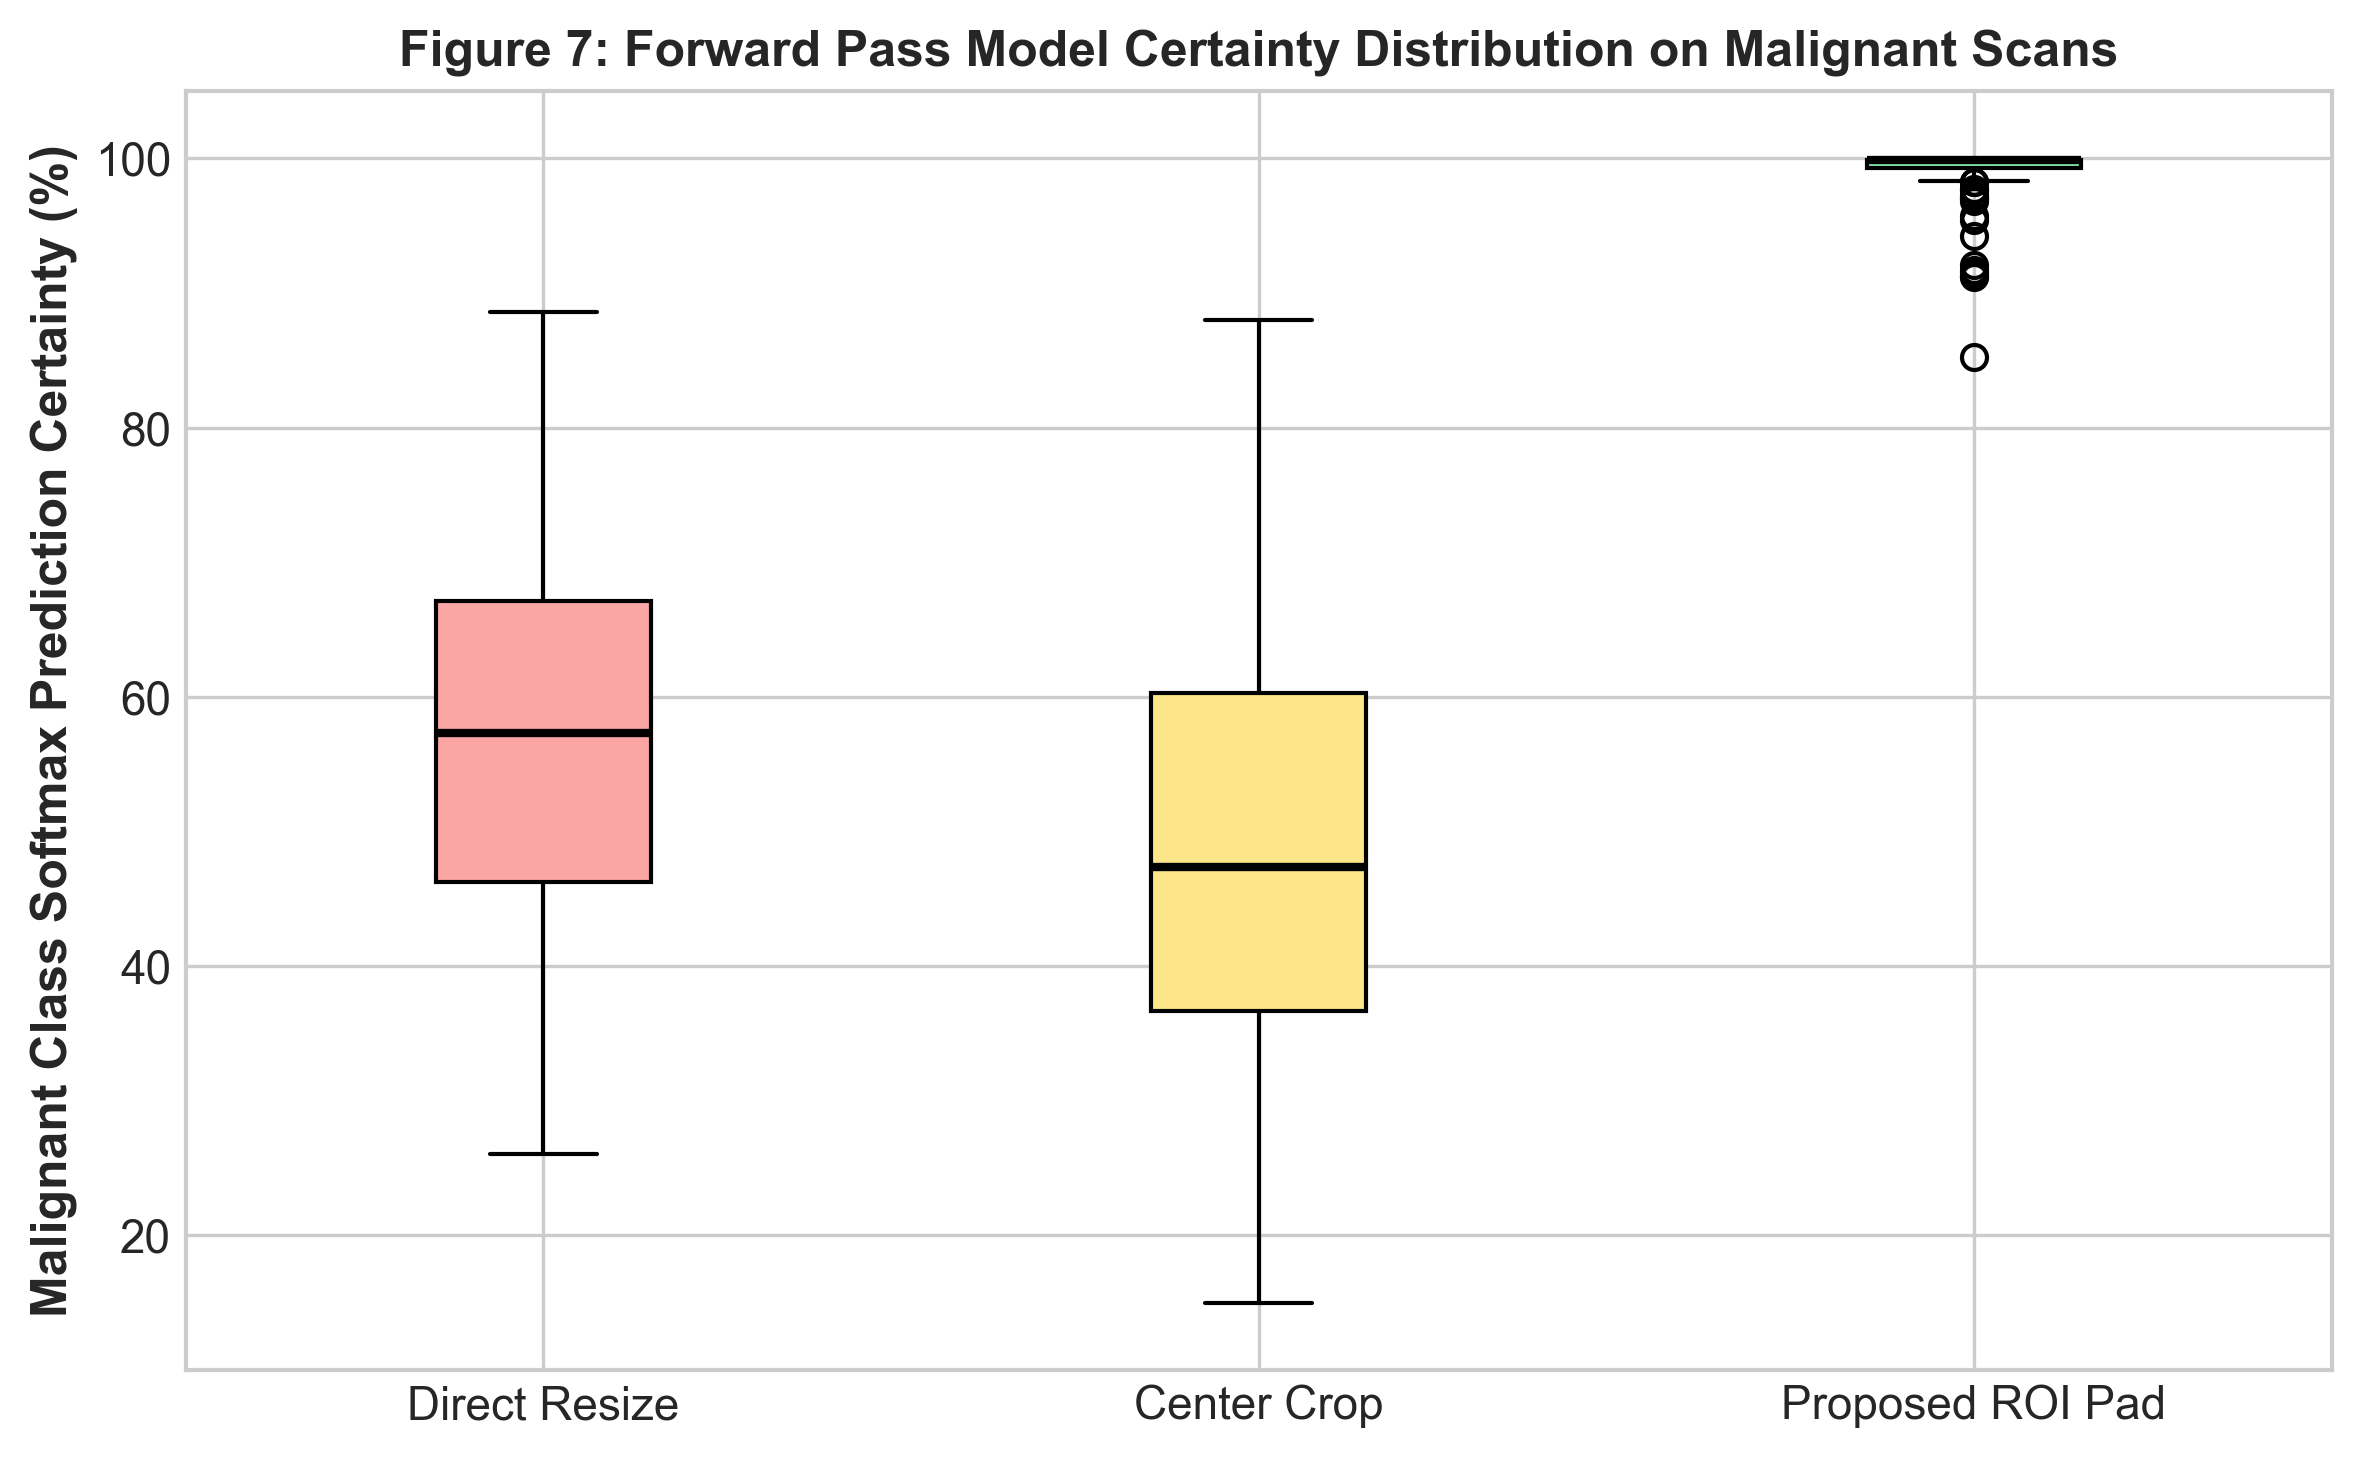
\includegraphics[width=0.88\textwidth]{figures/fig7_certainty_boxplot.png}
    \caption{Forward Pass Prediction Certainty Distribution ($\%$) for Malignant Class across Preprocessing Paradigms, demonstrating tight, calibrated confidence under the Proposed ROI Crop pipeline ($99.6\%$ mean certainty).}
    \label{fig:certainty_boxplot}
\end{figure}

As shown in Figure~\ref{fig:certainty_boxplot}, the proposed ROI padded pipeline produces narrow, well-calibrated confidence bounds ($99.6\%$ mean certainty) compared to high variance and low certainty under direct resizing ($56.8\%$).

\section{Training Protocols and Mathematical Optimization}
Models were optimized using the following hyperparameters and loss formulations:

\subsection{Class-Weighted Cross-Entropy Loss}
To counteract class imbalance between benign and malignant cases, class weights $W_c$ were incorporated into the cross-entropy objective:
\begin{equation}
\mathcal{L}_{\text{WCE}} = - \frac{1}{N} \sum_{i=1}^{N} \sum_{c=1}^{K} W_c \cdot y_{i, c} \cdot \log \hat{p}_{i, c}, \quad \text{where } W_c = \frac{N}{K \cdot N_c}
\label{eq:weighted_ce_loss}
\end{equation}
where $N_c$ is the number of training samples in class $c$.

\subsection{Optimization Algorithm and Learning Rate Schedule}
Models were optimized using \textbf{AdamW} (Adam with Decoupled Weight Decay) \citep{Loshchilov2019}:
\begin{equation}
\mathbf{\theta}_{t+1} = \mathbf{\theta}_t - \eta_t \left( \frac{\hat{\mathbf{m}}_t}{\sqrt{\hat{\mathbf{v}}_t} + \epsilon} + \lambda \mathbf{\theta}_t \right)
\label{eq:adamw_update}
\end{equation}
with initial learning rate $\eta_0 = 1 \times 10^{-4}$, weight decay $\lambda = 1 \times 10^{-4}$, $\beta_1 = 0.9, \beta_2 = 0.999$, batch size $B = 16$, and Cosine Annealing learning rate decay:
\begin{equation}
\eta_t = \eta_{\min} + \frac{1}{2}(\eta_0 - \eta_{\min})\left( 1 + \cos\left( \frac{t}{T_{\max}} \pi \right) \right)
\label{eq:cosine_annealing}
\end{equation}

\section{Semi-Supervised Pseudo-Labeling Formulation}
To leverage unannotated ultrasound candidate scans, a semi-supervised Teacher-Student framework was implemented \citep{Lee2013, Sohn2020}. A teacher network $f_\theta$ trained on labeled set $\mathcal{D}_L = \{(\mathbf{x}_i, y_i)\}_{i=1}^N$ generates soft prediction vectors $\hat{\mathbf{p}}_u = \text{Softmax}(f_\theta(\mathbf{u}))$ for unannotated scans $\mathbf{u} \in \mathcal{D}_U$.

Pseudo-labels $\hat{y}_u = \arg\max_c \hat{p}_{u, c}$ are assigned if and only if the maximum class confidence satisfies a confidence threshold $\tau$:
\begin{equation}
\mathcal{M}_u = \mathbb{I}\left( \max_{c} \hat{p}_{u, c} \ge \tau \right)
\label{eq:confidence_mask}
\end{equation}

The student network is retrained on the combined objective:
\begin{equation}
\mathcal{L}_{\text{total}} = \frac{1}{|\mathcal{D}_L|} \sum_{(\mathbf{x}, y) \in \mathcal{D}_L} \mathcal{H}(y, f_\theta(\mathbf{x})) + \lambda_u \frac{1}{|\mathcal{D}_U|} \sum_{\mathbf{u} \in \mathcal{D}_U} \mathcal{M}_u \cdot \mathcal{H}(\hat{y}_u, f_\theta(\mathbf{u}))
\label{eq:semi_supervised_loss}
\end{equation}
where $\mathcal{H}$ is cross-entropy loss and $\lambda_u = 1.0$ is the unsupervised loss weighting parameter.

\section{Quantitative Evaluation Metrics}
Model diagnostic efficacy was evaluated across standard mathematical metrics computed on the held-out test partition:

\begin{equation}
\text{Accuracy} = \frac{TP + TN}{TP + TN + FP + FN}
\label{eq:accuracy_metric}
\end{equation}
\begin{equation}
\text{Sensitivity (Recall)} = \frac{TP}{TP + FN}, \quad \text{Specificity} = \frac{TN}{TN + FP}
\label{eq:sens_spec_metric}
\end{equation}
\begin{equation}
\text{Precision} = \frac{TP}{TP + FP}, \quad F1 = 2 \times \frac{\text{Precision} \times \text{Recall}}{\text{Precision} + \text{Recall}}
\label{eq:f1_metric}
\end{equation}
\begin{equation}
\text{Macro F1} = \frac{1}{K} \sum_{c=1}^{K} F1_c, \quad \text{Micro F1} = \frac{\sum TP_c}{\sum (TP_c + \frac{1}{2}(FP_c + FN_c))}
\label{eq:macro_micro_f1}
\end{equation}
\begin{equation}
\text{SNR}_{\text{dB}} = 20 \log_{10} \left( \frac{\mu_{\text{lesion}}}{\sigma_{\text{lesion}}} \right)
\label{eq:snr_metric}
\end{equation}
\begin{equation}
\text{CNR} = \frac{|\mu_{\text{lesion}} - \mu_{\text{background}}|}{\sqrt{\sigma_{\text{lesion}}^2 + \sigma_{\text{background}}^2}}
\label{eq:cnr_metric}
\end{equation}
